\chapter{Realised work}

general procedure 

<diagram flowchart>


\section{First module : 3D map generation}


\subsection{Procedure}

=> est une introduction 

<diagram flowchart>


\subsection{Images}

An image is represented by a width, an heigth, colors (stocked in pixel values, i.e. positive integers), and a color model. A color model describes how the colors are represented, that is how many values should be used in order to represent a color. Multiples color models exist, for example : 
\begin{itemize}
	\item RGB, where a color is represented by the three primary colors (red, green and blue)
	\item CMY, where a color is represented by a combinaison of cyan, magenta and yellow colors
\end{itemize}

% https://en.wikipedia.org/wiki/Color_model 
% cours de jpeg 

We focused of three types of images : RGB, Grey and Monochromatic images. A grey image is an image where the pixels are represented in a grey scale by only one value, the grey value (which can have any integer values between 0 and 255 included). In other words, there is 256 possible colors in a grey images, which are all shade of grey. In a monochromatic image, only two colors are represented, black (with the value 0) and white (with the value 255).

Once we loaded an image in the RGB color model, we converted it into a grey image in order to reduce the number of information present in the image and lower the complexity. The monochromatic image were used in order to determinate edges and extract the objects in the image.

The grey value of a RGB pixel is determined by doing the average of the red, green and blue values. As for the monochromatic image, we first have to define a 
threshold value, then a pixel will be represented in black if it's grey value is strictly under the threshold, and in white otherwise (the equation \ref{eq:threshold} show it in a more mathematical point of view).

% https://en.wikipedia.org/wiki/Thresholding_(image_processing) 

\begin{equation} \label{eq:threshold}
mono_{threshold}(greyValue) = 
\begin{cases}
	BLACK & \text{if } greyValue < threshold\\
	WHITE & \text{otherwise} \\ 
\end{cases}
\end{equation}


We choosed to represent the grey and monochromatic image by a one matrix. 


.... 



<changer RGB image> 

\begin{figure}
	\centering 
	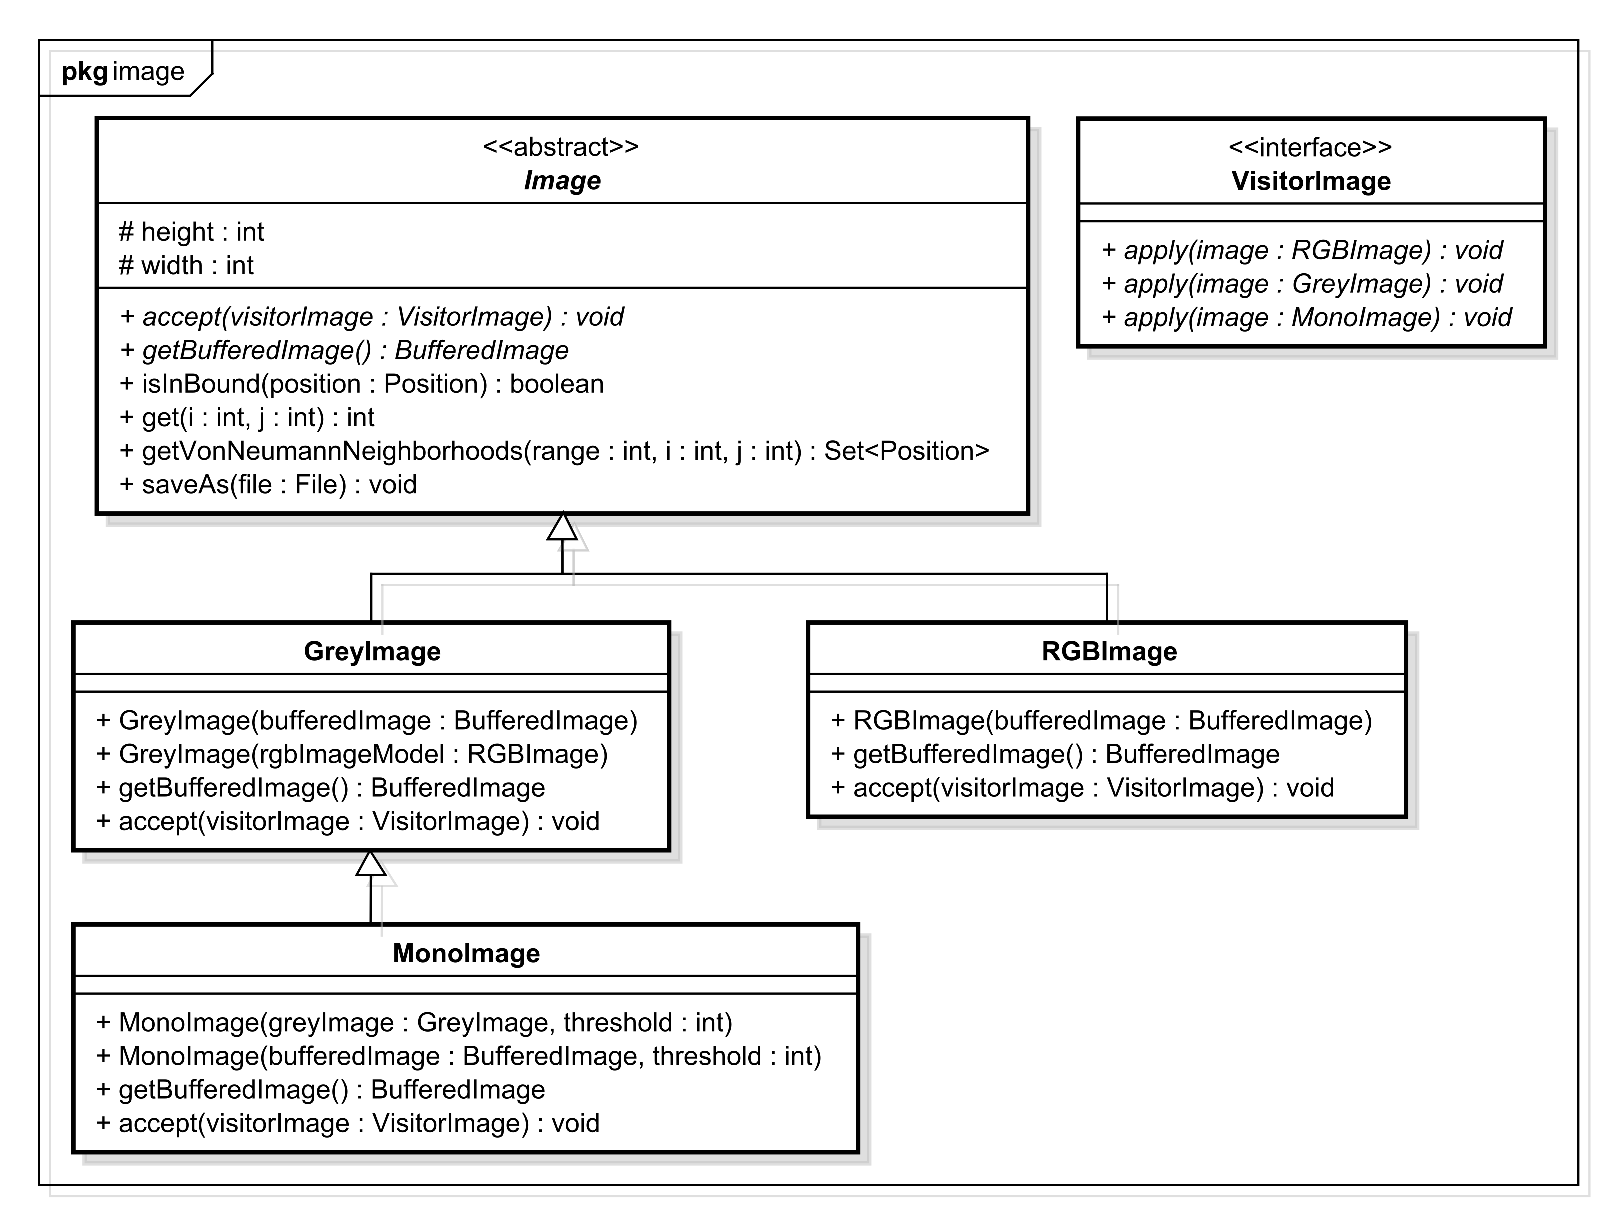
\includegraphics[width=0.75\textwidth]{images/diagrams/class_diagram_image}
	\caption{Image package class diagram}
	\label{fig:diagram:class:image}
\end{figure}


The visitor pattern was also used in order to facilitate the implementation of new processes (or algorithms) on a data structure without changing it. It does so by separating the algorithm and the data structure from each other. A new process (or algorithm) could be added by extending the VisitorImage class and implementing the apply method for each image subclasses. 

% https://en.wikipedia.org/wiki/Visitor_pattern 
% + cours 
% + book

\subsection{Rajan Tranform and Set Theoretic Rajan Transform}

We planned to use the Set Theoretic Rajan Transform (STRT) in our process but it wasn't possible due to some issues and imprecisions in the documentation concerning the STRT$^{-1}$. We wanted to use this transformation on an image mainly because it has noise removal properties.


The Set Theoretic Rajan Transform (STRT) correspond to the Rajan Transform (RT) applied on the sets domain. First I will present the forward rajan transform, and then it's application in the sets domain. Every equations, figures and explainations have been inspired by the following reference  \cite{bib:symbolic:RajanTransform}.

The rajan transform take a sequence of $2^{i}$ numbers (the number of elements of the sequence have to be a power of 2), transform it, and return another sequence of $2^{i}$ numbers. We will call $x(k)$ the input sequence, $X(k)$ the output sequence of the tranform, and $N$ the number of element in the sequence \cite{bib:symbolic:RajanTransform}. 


\begin{equation}
x = x(0), x(2), \cdots, x(k-1) \text{ where k is a power of 2}
\end{equation}

We will define two other sequences $g(k)$ and $h(k)$ as following : 
\begin{equation}
g(k) = x(k) + x(k + \frac{N}{2}) \text{ with } 0 \leq k \leq \frac{N}{2}
\end{equation}

\begin{equation}
h(k) = | x(k) - x(k - \frac{N}{2}) | \text{ with } \frac{N}{2} \leq k \leq N
\end{equation}


In other words, the sequence $x$ will be divided in two. Then we will sum the two first value of the subsequences (which will give us the results of $g(1)$), then the two seconds values (which is $g(2)$), then the thirds values, and so on until all the elements were processed. Then we will do the same operations but with a substraction instead (to get the sequence $h$).


This processus will then have to be repeated on the subsequences $g$ and $h$ separately. We can see here the recursive character of this transformation. The figure \ref{fig:diagram:flowchart:rajan} illustrate the rajan tranformation in a more procedural way, with a sequence of 4 elements. 

\begin{figure}[H]
	\centering
	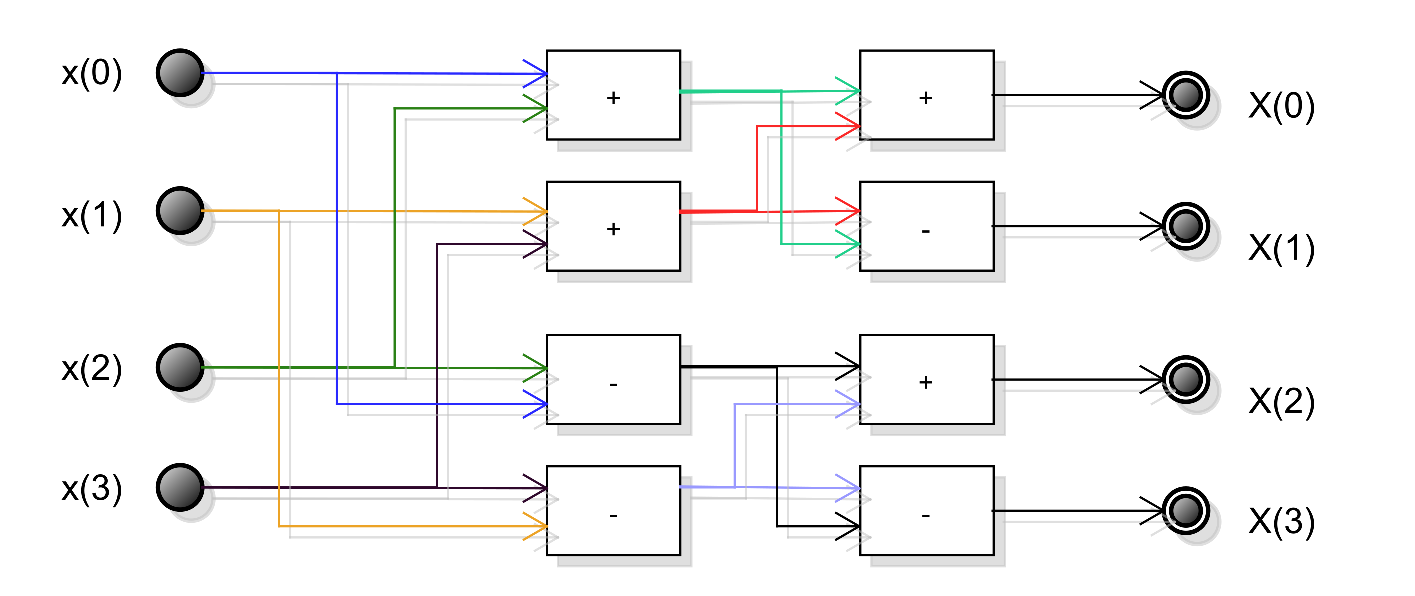
\includegraphics[width=0.7\textwidth]{images/diagrams/flowchart_rajan_transform}
	\caption{The forward Rajan Tranfform (RT)}
	\label{fig:diagram:flowchart:rajan}	
\end{figure}


The Set Theoretic Rajan Transform is the application of the Rajan Transform in the sets domain, and so instead of tranforming a sequence of numbers, it will tranform a sequence of sets, and return another sequence of sets (e.g. $x(1)$ and $X(1)$ wouldn't be numbers, but two sets). In the set domain, the addition correspond to the union, and the substraction to the difference of two sets.





\subsection{Filters}

\subsection{Cellular Automata algorithm}

\subsection{Morphology}

\subsection{Feature Extraction and Freeman Chain Code}

As we said before, in order to detect the different edges in th eimage, we used a filter edge detection, like sobel or canny. 

In order to extracts the differents features in the image, 


\subsection{Classification}

kmean > EM because show better results 
but - quand même (choisir nb classes + random with gravity center initialisation)


\subsection{GUI}

A Graphic User Interface has been developped during the project in order to see the results.... 


\section{Second module}

